\chapter{Thermal instability in homogeneous plasmas} \label{ch: thermal instability}

\graphicspath{{03-thermal_instability/figures/}}

\usespublishedwork{Most of this Chapter was published in ``Thermal instabilities: Fragmentation and field misalignment of filament fine structure", 2020, \aanda, 636, A112 \citep{claes2020}. N. Claes performed the simulations, analysed the data and wrote the manuscript. R. Keppens and C. Xia contributed to the revision of the paper. Some parts of this Chapter were also published in ``Thermal stability of magnetohydrodynamic modes in homogeneous plasmas", 2019, \aanda, 624, A96 \citep{claes2019}. N. Claes performed the simulations, analysed the data and wrote the manuscript; R. Keppens contributed to the revision of the paper.}

\section{Introduction}

\section{The physics of thermal instability}
As already mentioned in the previous Chapter, in non-adiabatic MHD the stability of the thermal (entropy) mode is strongly dependent on the heat-loss function $\HLF$, which in general depends on the usual thermodynamic quantities like density and temperature, and in some cases also on the magnetic field through the choice of heating function. In our formalism however, i.e. following Equation \eqref{eq: cooling_simple}, the heating term $\HLFheat$ is assumed to be constant such that $\HLF$ only depends on density and temperature. The latter dependence enters by means of the cooling curve $\HLFcool$, which are tabulated values resulting from detailed atomic and molecular calculations. Figure \ref{fig: coolingcurves} shows two of these tables as a function of temperature: the blue line denotes the curve given in \citet{colgan2008} (hereafter referred to as ``\jccorona''). The sharp drop near $10^4$ K is due to the ionisation of hydrogen, which essentially sets radiative cooling for lower temperatures to zero. The red curve on the other hand denotes the one given by \citet{schure2009} (hereafter referred to as ``\spexdm") and is extended to lower temperatures using \citet{dalgarno1972}.

\begin{figure}[t]
  \centering
  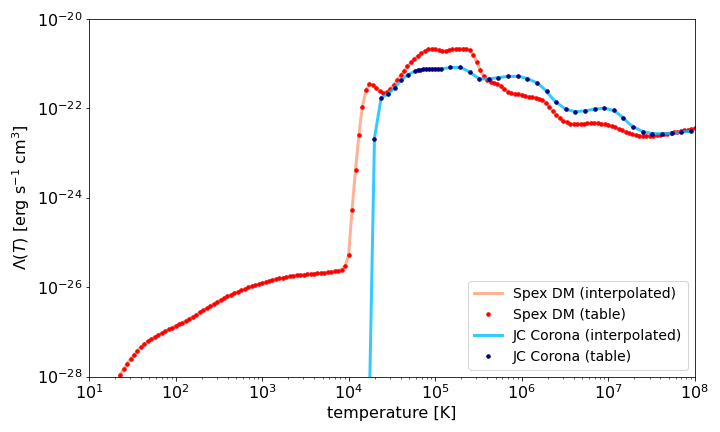
\includegraphics[width=\textwidth]{coolingcurves.png}
  \caption{
    Plots of two cooling curves $\HLFcool$ as a function of temperature. Red denotes the curve given by \citet{schure2009}, extended to low temperatures using \citet{dalgarno1972}. Blue denotes the curve given by \citet{colgan2008}.
  }
  \label{fig: coolingcurves}
\end{figure}

Now, suppose a plasma that gains energy from an external source (constant heating in this case) and looses energy to its surroundings through optically thin radiative cooling processes (cooling), but is in full thermal equilibrium such that these two contributions cancel each other out (i.e. $\HLF_0 = 0$). This thermal equilibrium state will only be maintained if the plasma is stable with respect to small perturbations, such that any deviation from this state is counteracted and the plasma returns to its initial configuration.

Now assume that this plasma is at a certain uniform temperature at which $\dHLFT$ is negative, that is, the value of $\HLFcool$ increases when temperature decreases. This is the case at e.g. two million Kelvin (see Figure \ref{fig: coolingcurves}) for both cooling curves. If this plasma is perturbed such that the temperature decreases slightly, $\dHLFT < 0$ implies that the radiative losses will increase and the plasma looses even more energy, decreasing the temperature even further. This process will happen relatively slow at first, but after a while the plasma reaches a point of no return and a \emph{catastrophic cooling phase will kick in}: the small, initial perturbation that lowered the temperature grows and leads to \emph{thermal instability}. Nature's tendency is to keep pressure equilibrium, and according to the ideal gas law $p = \rho T$ the initial drop in temperature is accompanied by an increase in density in an (in this case futile) attempt to restore pressure balance. This has an adverse effect on the plasma as the heat-loss function $\HLF$ as defined here is linearly dependent on density, meaning that a density increase leads to more energy losses. This, combined with the continuing drop in temperature leads to a runaway cooling process: the plasma density keeps increasing while the temperature keeps decreasing, giving rise to high-density, low-temperature regions.
A density perturbation can also give rise to thermal instability in the same manner as before: an increase in density implies a decrease in temperature or vice-versa (pressure balance), hence a temperature disturbance and the possibility to trigger instability. The effect of $\dHLFT$ on the growth rate of thermal instability is in general much stronger than $\dHLFrho$, except in regions where the heat-loss function has a relatively flat temperature dependence. In those cases the disturbance in density may actually be the dominant mechanism to trigger instability instead of temperature, where the density changes lead to cooling/heating variations.

The above discussion treats the case in which energy losses increase for decreasing temperature, but the reverse (i.e. $\dHLFT > 0$) may also give rise to instability. Here a drop in temperature decreases the energy losses, such that the heating term becomes dominant and heats up the plasma. A similar runaway process starts, where plasma density now decreases in an attempt to restore pressure equilibrium, lowering radiative losses even further. Generally speaking this process can also be referred to as ``thermal instability'', this time driven by heating. However, both cases give rise to both high density and low density plasma regions, such that we will not distinguish between the two.

Plasmas that are thermally stable will eventually return to thermal equilibrium after small perturbations. Due to the strong link between stability and $\dHLFT$, this will mainly happen in regions where the temperature dependence is minor, that is, for flat regions in the cooling curves. One such region may be just below $10^5$ K on Figure \ref{fig: coolingcurves}: here a small perturbation will only lead to a minor change in heating and cooling, such that the system has enough time to counteract the imbalance before the runaway reaction occurs. This may not be sufficient for perturbations that are large enough however, due to the delicate interplay between the heating and cooling terms, such that they might still be able to trigger instability.

If thermal conduction is also present then this will \emph{always} have a stabilising effect on the thermal instability. Initial temperature perturbations will be smoothened out due to thermal conduction effects, and even if the runaway cooling process has already started it will try and continue to do so. Generally speaking this stabilising behaviour will lead to a reduction of the thermal instability growth rate, but actually \emph{preventing} instability will only occur in a few select cases. The high anisotropy of thermal conduction plays a major role in magnetised plasmas as the effect is several orders of magnitude stronger parallel to the magnetic field lines than across, allowing for strong temperature gradients across field lines (and hence large $\dHLFT$ values). This implies that the direction of the wave vector is important, since perturbations more parallel to the magnetic field will be strongly stabilised, while wave vectors (near) perpendicular to the field lines will undergo almost no stabilisation by thermal conduction.

All of the above, which assumes a plasma at uniform temperature and a constant heating term, is ideal to get an intuitive feeling what thermal instability is and how it originates. In reality however things are much more complicated: the plasma is certainly not uniform, and in general the heat-loss function will have a complicated dependency on other (thermodynamic) variables. This implies that the process of thermal instability is much more intricate in fully realistic plasmas with regard to (in)stability, but the general idea holds: an unstable thermal mode triggers a runaway radiative cooling reaction, which in turn leads to high-density, low-temperature condensations.


\section{Growth rates of non-adiabatic MHD modes}

\section{Thermal instability and nonlinear fragmentation}
\subsection{Numerical setup}
\subsection{Synthetic views}
\subsection{Thermal instability onset in 2D}
\subsection{Thermal instability onset in 3D}

\section{Implications and the road ahead}
\cleardoublepage
